\chapter{Kajian Pustaka}

\section{Kerusakan Permukaan Jalan dan Dataset N-RDD2024}
Kerusakan permukaan jalan merupakan indikator utama dari penurunan kualitas perkerasan infrastruktur transportasi yang berdampak langsung pada keselamatan pengguna jalan. Secara umum, kerusakan jalan struktural diklasifikasikan ke dalam empat kategori utama, yaitu retak memanjang (\textit{longitudinal crack}/D00), retak melintang (\textit{transverse crack}/D10), retak buaya (\textit{alligator crack}/D20), dan lubang jalan (\textit{pothole}/D40). Klasifikasi standar ini menjadi landasan dalam pengembangan \textit{Road Damage Dataset 2022} (RDD2022), sebuah dataset global yang mengumpulkan puluhan ribu citra jalan dari berbagai negara untuk mendorong pengembangan deteksi jalan otomatis \cite{Arya2024846}.

% ==========================================
% GAMBAR: CONTOH LABEL KERUSAKAN JALAN
% ==========================================
\begin{figure}[H]
  \centering
  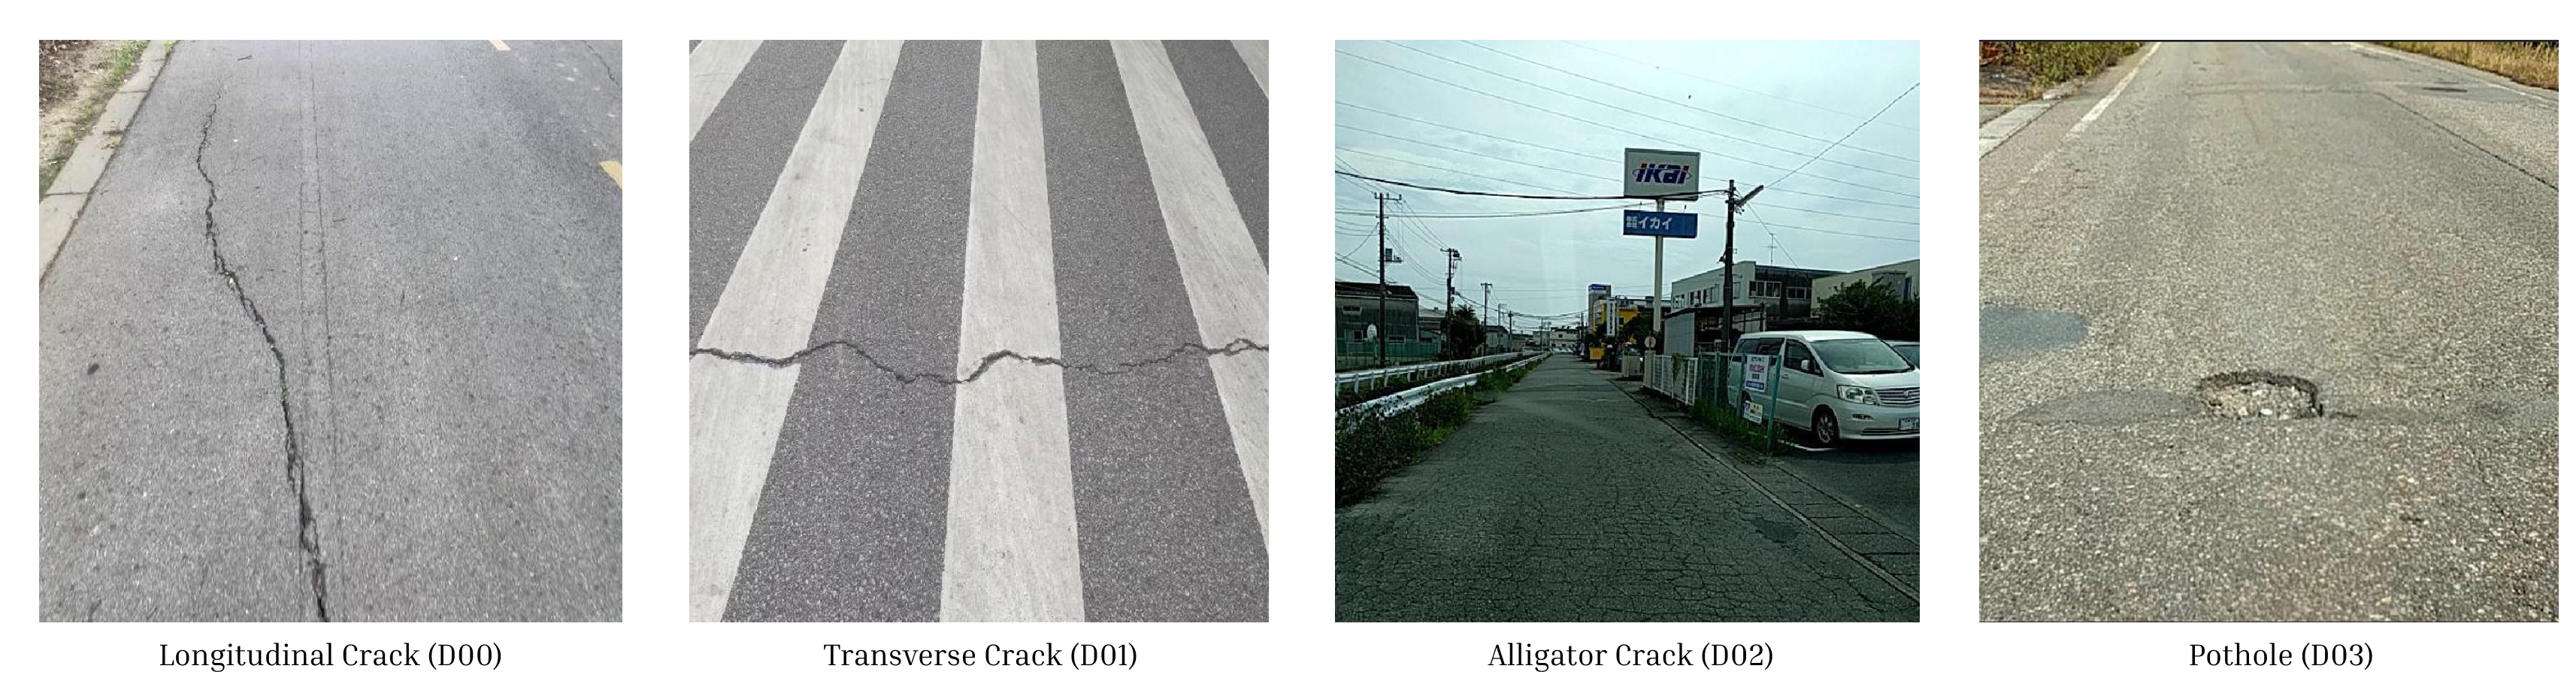
\includegraphics[width=\textwidth]{gambar/contoh_label_RDD.png}
  \caption{Contoh kerusakan jalan pada RDD2022 (D00, D10, D20, D40)}
  \label{fig:label_kerusakan_rdd}
\end{figure}

Meskipun RDD2022 telah memberikan kontribusi besar, dataset ini memiliki keterbatasan karena hanya berfokus pada kerusakan struktural utama dan mengabaikan elemen permukaan jalan lain yang memiliki kemiripan visual. Matouq dkk. menemukan bahwa mayoritas sistem deteksi kerusakan jalan sering kali gagal dan menghasilkan tingkat \textit{false positive} yang tinggi karena algoritma tidak mampu membedakan lubang jalan asli dengan elemen infrastruktur lain seperti penutup saluran air (\textit{manhole cover}) dan tambalan aspal (\textit{patching}) \cite{matouq2024ai}. Hal ini diperkuat oleh temuan Shi, yang mengonfirmasi bahwa penutup saluran air sangat sering dideteksi secara keliru sebagai lubang jalan, sehingga objek pengecoh tersebut mutlak perlu dianotasi secara terpisah saat melatih model \cite{Shi_2026}. Sejalan dengan tantangan tersebut, Kaya dan \c{C}odur memperkenalkan dataset N-RDD2024, sebuah perluasan dari RDD2022 yang menambahkan 10 kelas anomali dan cacat permukaan, termasuk kelas penutup saluran air (D70) dan jalan bertambal (D80) \cite{kaya2024nrdd2024}. Dalam konteks deteksi objek, kelas-kelas tambahan ini sangat krusial untuk difungsikan sebagai kelas pengecoh. Dengan melatih model untuk mengenali kelas D70 dan D80 secara eksplisit bersamaan dengan kelas kerusakan asli, model dapat belajar membedakan fitur visual yang mirip sehingga mampu menekan tingkat kesalahan deteksi di kondisi jalan nyata \cite{matouq2024ai, Shi_2026}.

Di sisi lain, pemanfaatan kelas yang beragam memunculkan tantangan baru berupa ketimpangan distribusi jumlah sampel latih (\textit{class imbalance}). Pada jalanan nyata, kerusakan berupa lubang jalan (\textit{pothole}) secara inheren memiliki frekuensi kemunculan yang jauh lebih sedikit dibandingkan dengan retakan memanjang atau melintang. Zeng dan Zhong membuktikan bahwa ketimpangan ini menyebabkan akurasi deteksi kelas lubang jalan (D40) pada model standar seperti YOLOv8 sering kali menjadi yang paling rendah, yang berujung pada terjadinya \textit{missed detection} (kegagalan deteksi) yang berulang \cite{Zeng2024}.  Oleh karena itu, arsitektur \textit{deep learning} yang digunakan memerlukan strategi khusus penanganan ketimpangan kelas pada tahap pelatihan, agar sensitivitas model terhadap kelas minoritas dapat tetap terjaga.

\section{\textit{You Only Look Once} (YOLO)}
Algoritma \textit{You Only Look Once} (YOLO) merupakan salah satu terobosan paling signifikan dalam bidang visi komputer yang diklasifikasikan sebagai detektor objek satu tahap (\textit{one-stage detector}) \cite{redmon2016you}. Berbeda dengan algoritma dua tahap (\textit{two-stage detector}) yang memerlukan proses pembuatan proposal wilayah (\textit{region proposal}) secara terpisah, YOLO mengubah rumusan masalah deteksi objek menjadi sebuah masalah regresi \textit{end-to-end} \cite{redmon2016you, Li2024}. Pendekatan ini memungkinkan jaringan saraf tiruan (\textit{neural network}) tunggal untuk memprediksi probabilitas kelas dan koordinat kotak pembatas (\textit{bounding box}) secara serentak dalam satu kali komputasi maju (\textit{single forward pass}), sehingga menghasilkan kecepatan inferensi yang sangat tinggi \cite{redmon2016you}.

Sejak pertama kali diperkenalkan oleh Joseph Redmon dkk. melalui iterasi YOLOv1, algoritma ini terus mengalami evolusi struktural yang pesat \cite{redmon2016you}. Redmon dkk. kemudian mengembangkan YOLOv2 (juga dikenal sebagai YOLO9000) dan YOLOv3, yang membawa peningkatan signifikan pada kemampuan deteksi objek melalui pengenalan jaringan residual, \textit{Spatial Pyramid Pooling} (SPP), dan \textit{Cross-Stage Partial Networks} (CSPNet) \cite{redmon2017yolo9000, redmon2018yolov3}. Evolusi arsitektur ini kemudian dilanjutkan oleh Bochkovskiy dkk. melalui peluncuran YOLOv4 pada tahun 2020, yang mengkonsolidasikan berbagai teknik optimasi mutakhir, termasuk augmentasi data \textit{Mosaic} dan modul atensi spasial, guna menawarkan detektor objek yang lebih optimal secara kecepatan maupun akurasi \cite{bochkovskiy2020yolov4}.

Iterasi baru dari keluarga algoritma ini, yaitu YOLOv8, dirilis oleh Ultralytics pada awal tahun 2023 dengan membawa pembaruan signifikan, termasuk penggunaan \textit{anchorless segmentation head} serta optimasi pada struktur jaringan \cite{Li2024}. Secara umum, arsitektur dasar jaringan YOLOv8 terbagi menjadi tiga komponen utama: \textit{Backbone} untuk ekstraksi fitur dari citra masukan, \textit{Neck} untuk melakukan fusi fitur multi-skala, dan \textit{Head} untuk menghasilkan prediksi akhir berupa lokasi, kelas, dan tingkat kepercayaan (\textit{confidence}) dari objek yang dideteksi \cite{Li2024, Zeng2024}.

% ==========================================
% GAMBAR 1: YOLOv8 STANDAR
% ==========================================
\begin{figure}[H]
  \centering
  % Gambar ini diambil dari Figure 3 pada Paper Li dkk. (2024)
  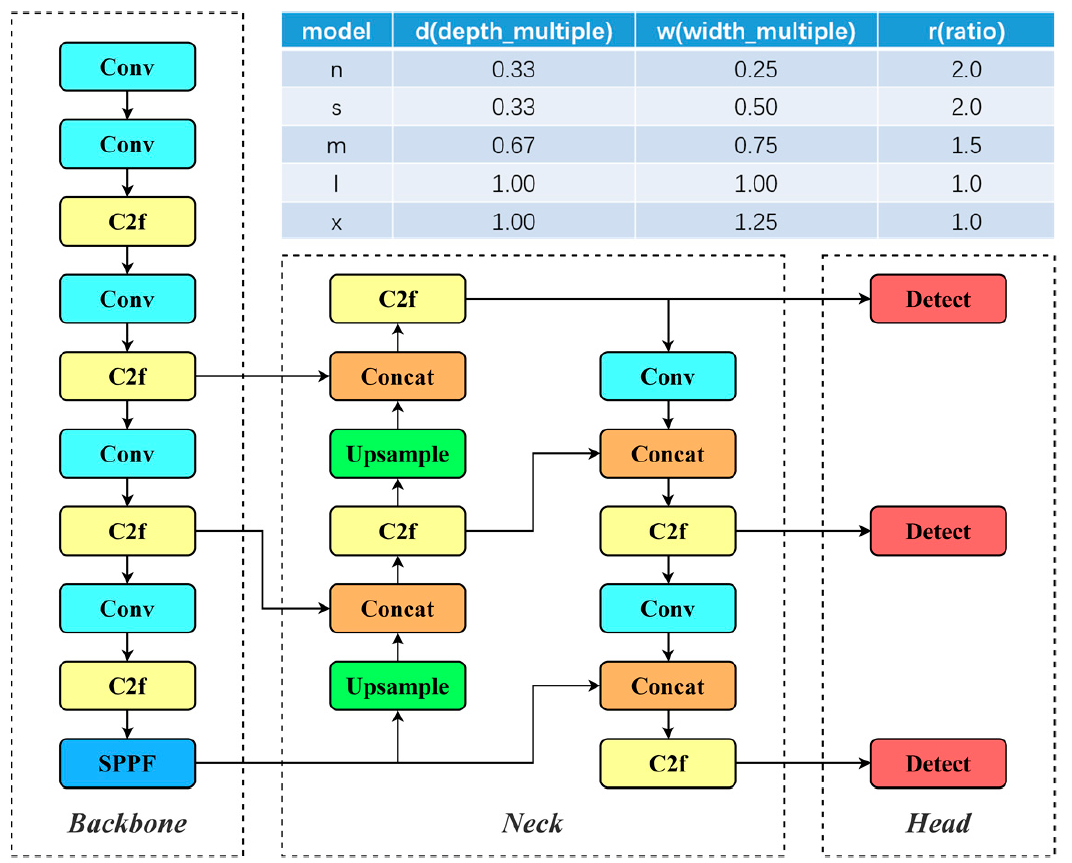
\includegraphics[width=0.85\textwidth]{gambar/arsitektur_yolov8_standar.png}
  \caption{Arsitektur Dasar Jaringan YOLOv8 (sumber: Li dkk., 2024 \cite{Li2024})}
  \label{fig:yolov8_standar}
\end{figure}

Algoritma YOLOv8 dirancang dengan tingkat fleksibilitas tinggi dan menyediakan lima varian berdasarkan skala kedalaman (\textit{depth}) dan lebar (\textit{width}) jaringan, yaitu YOLOv8n (nano), YOLOv8s (\textit{small}), YOLOv8m (\textit{medium}), YOLOv8l (\textit{large}), dan YOLOv8x (\textit{extra large}), sebagaimana yang diilustrasikan pada Gambar \ref{fig:yolov8_standar} \cite{Li2024}. Mengingat deteksi kerusakan jalan sering kali menuntut implementasi pada perangkat komputasi terbatas, varian yang paling ringan seperti YOLOv8n atau YOLOv8s menjadi kandidat \textit{baseline} yang paling ideal untuk meminimalkan beban komputasi.

\section{Modifikasi Arsitektur YOLO untuk Efisiensi}
Meskipun varian standar YOLOv8 telah memberikan performa yang baik, berbagai modifikasi struktural tingkat lanjut sering kali diperlukan untuk mengatasi tantangan spesifik pada citra jalan raya, seperti ukuran objek kerusakan yang sangat kecil (\textit{small objects}), latar belakang yang kompleks, serta keterbatasan memori perangkat.

Salah satu teknik modifikasi yang terbukti efektif adalah integrasi mekanisme atensi (\textit{attention mechanism}) ke dalam jaringan \cite{Wu2023, Li2024}. Mekanisme atensi, seperti \textit{Simple, Parameter-Free Attention Module} (SimAM) atau \textit{Convolutional Block Attention Module} (CBAM) \cite{woo2018cbam}, berfungsi untuk mengarahkan fokus model secara adaptif pada informasi visual yang krusial (seperti pola retakan tipis) sekaligus menekan gangguan (\textit{noise}) dari elemen visual latar belakang. Modul SimAM, misalnya, mampu menghitung bobot atensi tiga dimensi secara langsung dari fungsi energi neuron tanpa menambah beban parameter jaringan secara signifikan \cite{Li2024}.


% ==========================================
% GAMBAR 2: YOLOv8 MODIFIKASI
% ==========================================
\begin{figure}[H]
  \centering
  % Gambar ini diambil dari Figure 4 pada Paper Li dkk. (2024)
  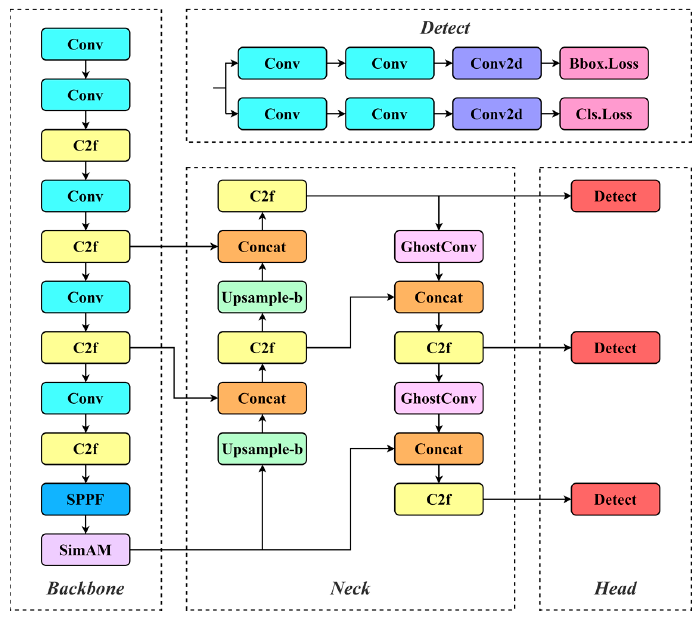
\includegraphics[width=0.85\textwidth]{gambar/arsitektur_yolov8_modifikasi.png}
  \caption{Contoh Modifikasi Arsitektur YOLOv8 yang Dioptimalkan untuk Efisiensi (sumber: Li dkk., 2024 \cite{Li2024})}
  \label{fig:yolov8_modifikasi}
\end{figure}

Selain mekanisme atensi, efisiensi model juga dapat ditingkatkan melalui modifikasi pada struktur konvolusi, sebagaimana diilustrasikan pada Gambar \ref{fig:yolov8_modifikasi}. Penggantian modul konvolusi standar pada bagian \textit{Neck} dengan \textit{Ghost Convolution} (\textit{GhostConv}) \cite{han2020ghostnet} mampu mereduksi redundansi fitur melalui operasi linear berbiaya rendah. Pendekatan ini secara drastis menurunkan jumlah parameter dan beban komputasi (GFLOPs) dengan tetap mempertahankan kemampuan ekstraksi fitur yang tangguh \cite{Zeng2024, Shi_2026}.

Di samping optimasi struktural, penanganan ketimpangan distribusi data (\textit{class imbalance}) mutlak diperlukan pada tahap pelatihan, terutama karena frekuensi kemunculan lubang jalan dan jalan bertambal jauh lebih sedikit dibandingkan dengan retakan memanjang dan buaya. Untuk mengatasi masalah ini secara stabil pada pelatihan presisi campuran (\textit{Automatic Mixed Precision} / AMP), pendekatan pembobotan kelas adaptif berbasis \textit{Effective Number of Samples} yang diperkenalkan oleh Cui dkk. \cite{cui2019class} diadopsi. Metode ini menghitung volume ruang fitur efektif yang dicakup oleh $n$ sampel menggunakan formulasi:
\begin{equation}
  E_n = \frac{1 - \beta^n}{1 - \beta}
\end{equation}
dengan $\beta \in [0, 1)$ sebagai hiperparameter yang merepresentasikan probabilitas tumpang tindih fitur. Bobot kerugian untuk setiap kelas $i$ kemudian dinormalisasi sebagai proporsi terbalik dari volume efektifnya:
\begin{equation}
  W_i = \frac{1 - \beta}{1 - \beta^{n_i}}
\end{equation}
Pendekatan ini mencegah ledakan bobot numerik ekstrem yang kerap terjadi pada skema pembobotan frekuensi terbalik mentah (\textit{inverse class frequency}), sehingga menjaga kestabilan konvergensi gradien tanpa mengabaikan penalti pada kelas minoritas \cite{cui2019class}. Penggabungan teknik atensi, konvolusi ringan, dan pembobotan kerugian efektif ini menjadi landasan kokoh bagi rancangan model deteksi yang tangguh dan seimbang.


\section{\textit{Domain Shift} dan Evaluasi \textit{Zero-Shot}}
Pengembangan model deteksi kerusakan jalan secara global sering dihadapkan pada masalah \textit{domain shift}, yaitu fenomena penurunan performa drastis ketika model yang dilatih pada dataset suatu wilayah diuji di wilayah lain \cite{Arya2024846}. Tantangan ini diyakini akan menjadi semakin kompleks ketika sistem deteksi diimplementasikan di Indonesia. Penelitian Hugo dkk. menunjukkan bahwa meskipun model telah dilatih secara spesifik menggunakan dataset jalanan lokal Indonesia, performa deteksinya masih tertahan pada tingkat moderat (F1-Score 59,7\%) \cite{hugo2025efficientdet}. Keterbatasan tersebut utamanya dipicu oleh tingginya kompleksitas fitur visual jalanan lokal serta kesulitan model dalam melakukan generalisasi pada data baru (\textit{unseen data}) \cite{hugo2025efficientdet}. Berdasarkan fakta tersebut, penerapan model yang dilatih secara eksklusif menggunakan dataset global, tanpa adanya representasi infrastruktur Indonesia, berpotensi kuat mengalami degradasi akurasi akibat fenomena \textit{domain shift}.


Untuk mengukur ketangguhan model secara objektif dalam menghadapi masalah tersebut, diterapkan skenario pengujian \textit{zero-shot}, yaitu mengevaluasi model yang dilatih pada data global secara langsung pada data primer jalan lokal tanpa melakukan pembelajaran ulang (\textit{fine-tuning}). Pengujian \textit{zero-shot} ini sangat relevan untuk diimplementasikan karena proses pengumpulan dan penganotasian ulang data kerusakan jalan secara spesifik untuk kebutuhan \textit{fine-tuning} membutuhkan waktu yang lama dan sangat menguras tenaga (\textit{time-consuming and labor-intensive}) \cite{matouq2024ai}. Oleh karena itu, evaluasi \textit{zero-shot} menjadi tolok ukur yang paling efisien untuk mengukur kemampuan generalisasi murni dari arsitektur \textit{deep learning} sebelum diterapkan secara nyata pada sistem pemantauan di Indonesia.

\section{Penelitian Terkait}
Penelitian mengenai deteksi kerusakan jalan berbasis \textit{deep learning} telah banyak dilakukan. Beberapa penelitian terdahulu telah mengusulkan berbagai modifikasi arsitektur YOLO maupun penggunaan dataset yang beragam. Meskipun demikian, sebagian besar model masih memiliki keterbatasan ketika dihadapkan pada masalah \textit{domain shift} dan tingginya tingkat \textit{false positive} akibat elemen pengecoh di jalan raya. Rincian perbandingan antara penelitian terdahulu (\textit{state-of-the-art}) dengan rencana penelitian ini dapat dilihat pada Tabel \ref{tab:penelitian_terkait}.

\small
\renewcommand{\arraystretch}{1.3}
\begin{longtable}{>{\raggedright}p{1.4cm}>{\raggedright}p{3.3cm}>{\raggedright\arraybackslash}p{7.8cm}}
  \caption{Kekurangan dan Kelebihan Penelitian Deteksi Kerusakan Jalan}\label{tab:penelitian_terkait}                                                                                                                                                                                                                                                                                                                                                                                                                             \\
  \hline
  \textbf{Sumber}             & \textbf{Metode \& Dataset}                                                                                                  & \textbf{Kelebihan \& Kekurangan}                                                                                                                                                                                                                                                                                                                                    \\
  \hline
  \endfirsthead
  \hline
  \textbf{Sumber}             & \textbf{Metode \& Dataset}                                                                                                  & \textbf{Kelebihan \& Kekurangan}                                                                                                                                                                                                                                                                                                                                    \\
  \hline
  \endhead
  \hline
  \endfoot
  \cite{Li2024}               & \textbf{Metode:} RDD-YOLO (YOLOv8 + SimAM + GhostConv) \newline \textbf{Dataset:} RDD2022                                   & \textbf{Kelebihan:} \newline $\bullet$ Mencapai akurasi mAP yang tinggi dengan beban komputasi yang lebih efisien dibandingkan YOLOv8 standar. \newline \textbf{Kekurangan:} \newline $\bullet$ Belum menguji efek \textit{domain shift} pada jalan di luar 6 negara dataset latih. \newline $\bullet$ Dataset tidak memuat anotasi kelas pengecoh secara spesifik. \\
  \hline
  \cite{Zeng2024}             & \textbf{Metode:} YOLOv8-PD (YOLOv8n + GhostNet) \newline \textbf{Dataset:} RDD2022                                          & \textbf{Kelebihan:} \newline $\bullet$ Arsitektur sangat ringan, berhasil menekan jumlah parameter komputasi hingga menjadi 2,3 juta parameter. \newline \textbf{Kekurangan:} \newline $\bullet$ Akurasi pada deteksi lubang jalan (D40) anjlok hingga 53,1\% dan sering gagal mendeteksi lubang kecil akibat ketimpangan kelas.                                    \\
  \hline
  \cite{matouq2024ai}         & \textbf{Metode:} YOLOv8 Instance Segmentation \newline \textbf{Dataset:} Data Custom Ohio                                   & \textbf{Kelebihan:} \newline $\bullet$ Membuktikan bahwa melatih kelas penutup saluran air dan tambalan jalan secara bersamaan terbukti menekan \textit{false positive}. \newline \textbf{Kekurangan:} \newline $\bullet$ Pengumpulan dan anotasi data mandiri memakan waktu dan membutuhkan komputasi yang sangat besar.                                           \\
  \hline
  \cite{hugo2025efficientdet} & \textbf{Metode:} EfficientDet-D0 \newline \textbf{Dataset:} Citra Jalan Indonesia                                           & \textbf{Kelebihan:} \newline $\bullet$ Menggunakan data jalan raya primer (lokal Indonesia) untuk evaluasi dan menggunakan fungsi \textit{loss} gabungan. \newline \textbf{Kekurangan:} \newline $\bullet$ Performa akurasi tertahan pada tingkat moderat (F1-Score 59,7\%) karena kesulitan model melakukan generalisasi fitur lokal.                              \\
  \hline
  \cite{Shi_2026}             & \textbf{Metode:} YOLO-LWD (GhostConv + ECA) \newline \textbf{Dataset:} Aug-RDD                                              & \textbf{Kelebihan:} \newline $\bullet$ Model sangat efisien secara komputasi dan menganotasi penutup saluran (\textit{manhole cover}) secara terpisah. \newline \textbf{Kekurangan:} \newline $\bullet$ Hanya divalidasi pada \textit{single domain} (jalan lokal Tiongkok), belum dievaluasi kemampuannya di negara lain.                                          \\
  \hline
  \textbf{Usulan}             & \textbf{Metode:} Evaluasi Komparatif YOLO \textit{lightweight} \newline \textbf{Dataset:} N-RDD2024 \& Jalan Raya Indonesia & \textbf{Kelebihan Rencana Penelitian:} \newline $\bullet$ Menggabungkan dataset global N-RDD2024 (dengan anotasi kelas pengecoh eksplisit) dan mengujinya secara \textit{zero-shot} langsung pada jalan Indonesia.                                                                                                                                                  \\
  \hline
\end{longtable}

Berdasarkan Tabel \ref{tab:penelitian_terkait}, terlihat bahwa sebagian besar model yang berkinerja tinggi dikembangkan menggunakan dataset global (seperti RDD2022) yang tidak mencakup kelas pengecoh secara eksplisit \cite{Li2024, Zeng2024}. Di sisi lain, penelitian yang telah menyoroti pentingnya kelas pengecoh seperti penutup saluran air dan tambalan aspal masih dievaluasi pada lingkungan yang terbatas (\textit{single domain}) \cite{matouq2024ai, Shi_2026}. Sementara itu, implementasi model deteksi secara langsung di Indonesia masih menunjukkan performa yang tertahan akibat kompleksitas fitur jalanan lokal \cite{hugo2025efficientdet}. Oleh karena itu, penelitian Tugas Akhir ini diusulkan untuk mengisi kesenjangan (\textit{research gap}) tersebut secara sistematis dengan melakukan evaluasi komparatif arsitektur YOLO \textit{lightweight} menggunakan dataset N-RDD2024, serta mengukur ketangguhan generalisasinya secara \textit{zero-shot} di domain jalan raya Indonesia.
